\section{Nicomachean Ethics - Book V}

            \subsection{Preamble - Two kinds of justice}

                Traditionally:

                    \begin{itemize}
                        \item Distributive justice
                        \item Rectificatory justice
                    \end{itemize}

                \subsubsection{Unjust or unequal}

                    Since the unjust person is unfair, or unequal, and what is unjust is unfair, or unequal, it is clear that there is a mean in respect of what is unfair, namely, what is fair, or equal. In any kind of action in which there is a more and a less, there is also an equal. So if what is unjust is unequal, what is just must be equal– something that everyone thinks, even without argument. Since what is equal is a mean, the just will be some sort of mean.

                \subsubsection{Mean}

                    Cowardice – Courage - Temerity

            \subsection{Four terms}

                Because equality requires at least two terms, what is just must be a mean, and equal, and relative, namely, just for certain people. And, in so far as it is a mean, it must be between certain extremes (excess and deficiency); in so far as it is equal, it must involve two terms; and in so far as it is just, it must be so for certain people. So what is just requires at least four terms: the persons for whom it is just are two, and the shares in which its justice consists are two.

                \begin{remark}[Unequal persons, unequal shares]
                    There will be the same level of equality between persons as between shares, because the shares will be in the same ratio to one another as the persons. For if the persons are not equal, they will not receive equal shares; in fact quarrels and complaints arise either when equals receive unequal shares in an allocation, or unequals receive equal shares.
                \end{remark}

                \subsubsection{Merit}

                    This is clear also from the principle of distribution according to merit. For everyone agrees that justice in distribution must be in accordance with some kind of merit… So the just is a sort of proportion…

            \subsection{Distributive Justice}

                 What is just will also involve at least four terms, and the ratio is the same, since the persons and the shares are divided in the same ratio. As the term A, then, is to the term B, so will C be to D, and consequently, in permutation, as A is to C, so B is to D. And so whole will bear the same ratio to whole. It is this combination which the distribution brings about, and, if the terms be united in this way, brings about justly.

                    \begin{align}
                        A:B = & \ C:D \\
                        A:C = & \ B:D
                    \end{align}

                    \begin{example}
                        \begin{align}
                            \text{First best poet} : \text{Second best poet} = & \ \text{Gold crown} : \text{Silver crown} \\
                            \text{First best poet} :\text{Gold crown}  = & \ \text{Second best poet} : \text{Silver crown}
                        \end{align}
                    \end{example}

                    \subsubsection{Geometrical proportion}

                        What is just in distribution, therefore, is the conjunction of the term A with the term C, and of the term B with the term D. And the just in this sense is a mean, and the unjust violates the proportion, since what is proportionate is a mean, and the just is proportionate. Mathematicians call this kind of proportion “geometrical”, because in geometrical proportion what happens is that whole is to whole as each part is to each part.

                \subsection{Rectificatory Justice}

                    The other kind of justice is rectificatory, which is found in both voluntary and involuntary transactions. It belongs to a different species from that above. For the just in distribution of common property is always in accordance with the proportion stated above, since if the distribution is from common funds, it will be in the same ratio as are the corresponding investments to one another . And the injustice that is opposed to this kind of justice is what violates the proportion.

                    \subsubsection{Arithmetical proportion}

                        What is just in transactions is nevertheless a kind of equality, and what is unjust a kind of inequality, in accordance, however, not with that kind of proportion, but with arithmetical proportion.

                        \begin{remark}[Equal persons]
                            For it makes no difference whether it is a good person who has defrauded a bad or a bad person a good, nor whether it is a good or bad person that has committed adultery. The law looks only to the difference made by the injury, and treats the parties as equals, if one is committing injustice, and the other suffering it– that is, if one has harmed, and the other been harmed.
                        \end{remark}

                    \subsubsection{The Judge}

                        So the judge, since this kind of injustice is an inequality, tries to equalize it. For even when one party is struck, and the other strikes, or one kills, and the other is killed, the suffering and the action are divided unequally. The judge tries to equalize them with the penalty, decreasing the gain that has been made. For the word “gain” is generally employed in such cases, even if it is not appropriate for some of them, such as assault, and the same goes for the use of the word “loss” of the victim. At any rate, when the damage has been assessed, the one is called loss, the other gain.

                    \subsubsection{Loss and gain}

                        These names, “loss” and “gain”, are in fact derived from voluntary exchange. For having more than one’s share is called gaining, while having less than one had at the beginning is called losing– in buying and selling, for example, and other transactions in which the law has left people free to decide their own terms. But when neither party gets too much or too little, and both get what they gave, they say that they have what belongs to them, and that they neither lose nor gain. It follows that in voluntary transactions the just is a mean between some kind of gain and loss; it consists in having an equal amount both before and after the transaction.

                        \begin{remark}[Unequal parts]
                            This is why, when people are in dispute, they turn to a judge…. The judge restores equality. It is as if there were a line divided into unequal parts, and he takes away that by which the greater segment exceeds the half, and adds it to the smaller segment.
                        \end{remark}

            \subsection{Mean}

                What is equal is a mean between the greater and the less according to arithmetical proportion, because when a certain amount is subtracted from one of two equals and added to the other, the other exceeds the first by double that amount; for if the amount had been subtracted, but not added to the other, it would have exceeded it by only once that amount. It therefore exceeds the mean by once the amount, and the mean exceeds by once the amount that from which the amount was subtracted.

                In this way, then, we shall work out what we must subtract from the party with more, and add to the party with less; for we must add to the party with less the amount by which the mean exceeds what he has, and subtract from the greatest quantity the amount by which it exceeds the mean.

                \begin{example}

                    Let the lines AA', BB' and CC' be equal to one another.

                    \begin{center}
                        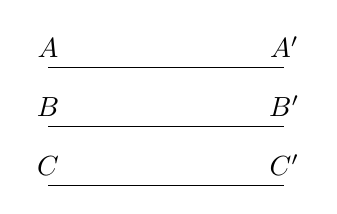
\begin{tikzpicture}[scale=0.75]
                          % Line for A--A'
                          \draw (0,0) -- (4,0);
                          \node[above]  at (0,0)   {$A$};
                          \node[above] at (4,0)   {$A'$};
                        
                          % Line for B--B'
                          \draw (0,-1) -- (4,-1);
                          \node[above]  at (0,-1)  {$B$};
                          \node[above] at (4,-1)  {$B'$};
                        
                          % Line for C--C'
                          \draw (0,-2) -- (4,-2);
                          \node[above]  at (0,-2)  {$C$};
                          \node[above] at (4,-2)  {$C'$};
                        \end{tikzpicture}
                    \end{center}
                    
                    \vspace{1em}

                    From the line AA', let the segment AE be subtracted:

                    \begin{center}
                        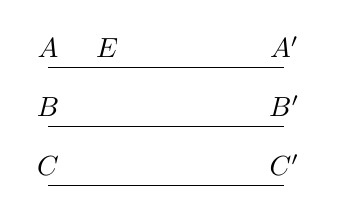
\begin{tikzpicture}[scale=0.75]
                          % A--E--A'
                          \draw (0,0) -- (4,0);
                          \node[above]  at (0,0)   {$A$};
                          \node[above] at (1,0)   {$E$};  % Place E somewhere between A and A'
                          \node[above] at (4,0)   {$A'$};
                        
                          % B--B'
                          \draw (0,-1) -- (4,-1);
                          \node[above]  at (0,-1)  {$B$};
                          \node[above] at (4,-1)  {$B'$};
                        
                          % C--C'
                          \draw (0,-2) -- (4,-2);
                          \node[above]  at (0,-2)  {$C$};
                          \node[above] at (4,-2)  {$C'$};
                        \end{tikzpicture}
                    \end{center}
                    
                    \vspace{1em}

                    and the segment CD added to the line CC', so that the whole line DCC' exceeds the line EA' by the segment CD and the segment CF; thus it exceeds the line BB' by the segment CD.

                    \begin{center}
                        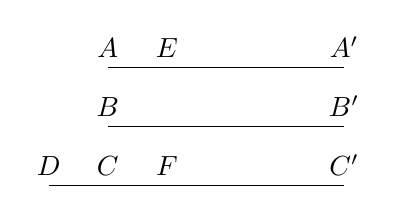
\begin{tikzpicture}[scale=0.75]
                          % A--E--A'
                          \draw (0,0) -- (4,0);
                          \node[above]  at (0,0)   {$A$};
                          \node[above] at (1,0)   {$E$};
                          \node[above] at (4,0)   {$A'$};
                        
                          % B--B'
                          \draw (0,-1) -- (4,-1);
                          \node[above]  at (0,-1)  {$B$};
                          \node[above] at (4,-1)  {$B'$};
                        
                          % D--C--F--C'
                          \draw (-1,-2) -- (4,-2);
                          \node[above]  at (-1,-2)  {$D$};
                          % Choose positions for C and F
                          \node[above] at (0,-2)  {$C$}; 
                          \node[above] at (1,-2)  {$F$};
                          \node[above] at (4,-2)  {$C'$};
                        \end{tikzpicture}
                    \end{center}
                    
                \end{example}

        \section{Two kinds of justice}

            \begin{definition}
                Distributive justice: (geometrical proportion) unequal people, unequal share
            \end{definition}

            \begin{definition}
                Rectificatory justice: (arithmetical proportion) equal people, correction of undue “gains”
            \end{definition}

                    \subsubsection{Loss and gain}

                        These names, “loss” and “gain”, are in fact derived from voluntary exchange. For having more than one’s share is called gaining, while having less than one had at the beginning is called losing– in buying and selling, for example, and other transactions in which the law has left people free to decide their own terms. But when neither party gets too much or too little, and both get what they gave, they say that they have what belongs to them, and that they neither lose nor gain. It follows that in voluntary transactions the just is a mean between some kind of gain and loss; it consists in having an equal amount both before and after the transaction.

                        \begin{remark}[Unequal parts]
        
                            This is why, when people are in dispute, they turn to a judge…. The judge restores equality. It is as if there were a line divided into unequal parts, and he takes away that by which the greater segment exceeds the half, and adds it to the smaller segment.
                            
                        \end{remark}

            \subsection{The Judge}

                So the judge, since this kind of injustice is an inequality, tries to equalize it. For even when one party is struck, and the other strikes, or one kills, and the other is killed, the suffering and the action are divided unequally. The judge tries to equalize them with the penalty, decreasing the gain that has been made. For the word “gain” is generally employed in such cases, even if it is not appropriate for some of them, such as assault, and the same goes for the use of the word “loss" of the victim. At any rate, when the damage has been assessed, the one is called loss, the other gain.

            \subsection{Loss and gain}

                These names, “loss” and “gain”, are in fact derived from voluntary exchange. For having more than one’s share is called gaining, while having less than one had at the beginning is called losing– in buying and selling, for example, and other transactions in which the law has left people free to decide their own terms. But when neither party gets too much or too little, and both get what they gave, they say that they have what belongs to them, and that they neither lose nor gain. It follows that in voluntary transactions the just is a mean between some kind of gain and loss; it consists in having an equal amount both before and after the transaction.

            \subsection{Transactions}

                \begin{definition}
                    Involuntary transactions (such as theft) that may require correction by a judge
                \end{definition}

                \begin{definition}
                    Voluntary transaction (such as exchange) that are based on reciprocity
                \end{definition}

                \subsubsection{Reciprocity}

                    Some hold that reciprocity is just without qualification. This was the claim of the Pythagoreans, since they defined, without qualification, what is just as reciprocity with another. Reciprocity, however, fits neither distributive nor rectificatory justice… For example, if a person in authority strikes someone, he should not be struck in return, but if someone has wounded an official, he should not only be struck in return, but receive an additional punishment.

                \subsubsection{Proportionate reciprocation}

                    When people associate with one another for the purpose of exchange, however, this kind of justice– reciprocity in accordance with proportion, not equality– is what binds them together, since a city is kept together by proportionate reciprocation. For people seek to return either evil for evil– otherwise they feel like slaves– or good for good– otherwise no exchange takes place, and it is exchange that holds them together.

        \section{A third kind of justice}

            \begin{quote}
                \textit{antipeponthos kat' analogían}
            \end{quote}

            \begin{quote}
                \textit{reciprocity in accordance with proportion}\footnote{not in accordance with equality, as instead for rectificatory justice}
            \end{quote}

            \begin{equation}
                \text{proportional reciprocity} \neq \ \text{rectificatory justice (equal reciprocity)}
            \end{equation}

            \subsection{Proportionate reciprocation}

                When people associate with one another for the purpose of exchange, however, this kind of justice– reciprocity in accordance with proportion, not equality– is what binds them together, since a city is kept together by proportionate reciprocation. For people seek to return either evil for evil– otherwise they feel like slaves– or good for good– otherwise no exchange takes place, and it is exchange that holds them together.

                It is a diagonal conjunction that produces proportionate reciprocation. Let A represent a builder, B a shoemaker, C a house, and D a shoe. The builder must get from the shoemaker his work, and must hand over his own in return. If, first, proportionate equality is established, and then reciprocation takes place, the result we mentioned will follow. If not, there is no equality, and the bargain falls through, since there is no reason why what one produces should not be more valuable than what the other produces, and the products must therefore be equated.

                \subsubsection{Loss and gain}

                    These names, “loss” and “gain”, are in fact derived from voluntary exchange. For having more than one’s share is called gaining, while having less than one had at the beginning is called losing– in buying and selling, for example, and other transactions in which the law has left people free to decide their own terms. But when neither party gets too much or too little, and both get what they gave, they say that they have what belongs to them, and that they neither lose nor gain. It follows that in voluntary transactions the just is a mean between some kind of gain and loss; it consists in having an equal amount both before and after the transaction.

                \subsubsection{Proportionate reciprocation}

                    When people associate with one another for the purpose of exchange, however, this kind of justice– reciprocity in accordance with proportion, not equality– is what binds them together, since a city is kept together by proportionate reciprocation. For people seek to return either evil for evil– otherwise they feel like slaves– or good for good– otherwise no exchange takes place, and it is exchange that holds them together.

            \subsection{Measure}

                This is why everything that is exchanged must be in some way commensurable. This is where money comes in; it functions as a kind of mean, since it is a measure of everything in a way that can also measure excess and deficiency. It can tell us, for example, how many shoes are equal to a house or some food. Then, as builder is to shoemaker, so must the number of shoes be to a house. For without this, there can be no exchange and no association; and it will not come about unless the products are in some sense equal.

                \subsubsection{Money}

                    So money makes things commensurable as a measure does, and equates them; for without exchange there would be no association between people, without equality no exchange, and without commensurability no equality… So there must be some one standard, and it must be on an agreed basis– which is why money is called \textit{nomisma}.    

                    Money makes all things commensurable, since everything is measured by money. Let A be a house, B ten minae, C a bed. A is half of B, if the house is worth, or equal to, five minae; and C, the bed, is worth one tenth of B. It is obvious, then, how many beds are equivalent to a house, namely, five. This is clearly how exchange took place before the existence of money <as mina>, since it makes no difference whether you pay five beds for a house, or as many minae as five beds. We have now described the nature of what is just and unjust.

                \subsubsection{Proportional Reciprocity}

                    …it is not two doctors who associate for exchange, but rather a doctor and a farmer, and, in general, people who are different and unequal, and must be made equal.

        \section*{L2 - Conclusions}

            In exchange as described by Aristotle, the differences are not treated in different ways as in the case of distributive justice, but are brought into equality, and this equalisation occurs in such a way that the initial differences are not rectified or annulled, as in the case of rectificatory justice, but on the contrary are recognised as such.
            